% !TeX spellcheck = en_US
\documentclass[12pt]{article}

\usepackage{fancyhdr} % Required for custom headers
\usepackage{lastpage} % Required to determine the last page for the footer
\usepackage{extramarks} % Required for headers and footers
\usepackage[usenames,dvipsnames]{color} % Required for custom colors
\usepackage{graphicx} % Required to insert images
\usepackage{listings} % Required for insertion of code
\usepackage{courier} % Required for the courier font
\usepackage{lipsum} % Used for inserting dummy 'Lorem ipsum' text into the template
\usepackage{amsmath}
\usepackage{caption}
\usepackage{multirow}
\usepackage{graphicx}
\usepackage{amssymb}
\usepackage{caption}
\usepackage{subcaption}
\usepackage{algorithm}
\usepackage{algpseudocode}
\usepackage{epstopdf}
\usepackage[dvipsnames]{xcolor}
% Margins
\topmargin=-0.45in
\evensidemargin=0in
\oddsidemargin=0in
\textwidth=6.5in
\textheight=9.0in
\headsep=0.25in
\headheight=15.0pt


\linespread{1.1} % Line spacing

% Set up the header and footer
\pagestyle{fancy}
\lhead{\hmwkAuthorName} % Top left header
\chead{\hmwkClass: \hmwkTitle} % Top center head
\cfoot{} % Bottom center footer
\rfoot{Page\ \thepage\ of\ \protect\pageref{LastPage}} % Bottom right footer
\renewcommand\headrulewidth{0.4pt} % Size of the header rule
\renewcommand\footrulewidth{0.4pt} % Size of the footer rule

\setlength\parindent{0pt} % Removes all indentation from paragraphs

%----------------------------------------------------------------------------------------
%	DOCUMENT STRUCTURE COMMANDS
%	Skip this unless you know what you're doing
%----------------------------------------------------------------------------------------

% Header and footer for when a page split occurs within a problem environment
\newcommand{\enterProblemHeader}[1]{
	\nobreak\extramarks{#1}{#1 continued on next page\ldots}\nobreak
	\nobreak\extramarks{#1 (continued)}{#1 continued on next page\ldots}\nobreak
}

% Header and footer for when a page split occurs between problem environments
\newcommand{\exitProblemHeader}[1]{
	\nobreak\extramarks{#1 (continued)}{#1 continued on next page\ldots}\nobreak
	\nobreak\extramarks{#1}{}\nobreak
}

\setcounter{secnumdepth}{0} % Removes default section numbers
\newcounter{homeworkProblemCounter} % Creates a counter to keep track of the number of problems

\newcommand{\homeworkProblemName}{}
\newenvironment{homeworkProblem}[1][Problem \arabic{homeworkProblemCounter}]{ % Makes a new environment called homeworkProblem which takes 1 argument (custom name) but the default is "Problem #"
	\stepcounter{homeworkProblemCounter} % Increase counter for number of problems
	\renewcommand{\homeworkProblemName}{#1} % Assign \homeworkProblemName the name of the problem
	\section{\homeworkProblemName} % Make a section in the document with the custom problem count
	\enterProblemHeader{\homeworkProblemName} % Header and footer within the environment
}{
	\exitProblemHeader{\homeworkProblemName} % Header and footer after the environment
}

\newcommand{\problemAnswer}[1]{ % Defines the problem answer command with the content as the only argument
	\noindent\framebox[\columnwidth][c]{\begin{minipage}{0.98\columnwidth}#1\end{minipage}} % Makes the box around the problem answer and puts the content inside
}

\newcommand{\homeworkSectionName}{}
\newenvironment{homeworkSection}[1]{ % New environment for sections within homework problems, takes 1 argument - the name of the section
	\renewcommand{\homeworkSectionName}{#1} % Assign \homeworkSectionName to the name of the section from the environment argument
	\subsection{\homeworkSectionName} % Make a subsection with the custom name of the subsection
	\enterProblemHeader{\homeworkProblemName\ [\homeworkSectionName]} % Header and footer within the environment
}{
	\enterProblemHeader{\homeworkProblemName} % Header and footer after the environment
}

%----------------------------------------------------------------------------------------
%	NAME AND CLASS SECTION
%----------------------------------------------------------------------------------------

\newcommand{\hmwkTitle}{Assignment\ \#5} % Assignment title
\newcommand{\hmwkClass}{Advanced Image Processing} % Course/class
\newcommand{\hmwkClassInstructor}{Jones} % Teacher/lecturer
\newcommand{\hmwkAuthorName}{Shikhar Vashishth} % Your name
\newcommand{\hmwkAuthorID}{M.Tech CSA - 13374} % Your ID

%----------------------------------------------------------------------------------------
%	TITLE PAGE
%----------------------------------------------------------------------------------------

\title{
	\vspace{2in}
	\textmd{\textbf{\hmwkClass}}\\ 
	\textmd{\textbf{\hmwkTitle}}\\
	\vspace{3in}
}

\author{\textbf{\hmwkAuthorName} \\ {\small \hmwkAuthorID}}
\date{} % Insert date here if you want it to appear below your name

%----------------------------------------------------------------------------------------

\begin{document}
	
	\maketitle
	\newpage
	
	\begin{homeworkProblem}
	\subsubsection{Spearman Rank Order Correlation Coefficients (SROCC):}
	\textbf{Metric 1 (MSE): }$0.782274$ \\
	\textbf{Metric 2 (SSIM): }$-0.903680$ \\ 
	\textbf{Metric 3 (CS): }$-0.90135$ \\ 
	\textbf{Metric 4 (MSE$_{mod}$): }$0.90135$ \\
	
	\subsubsection{Observations:}
	\begin{enumerate}
		\item We know from the definition of DMOS measure that smaller the value of DMOS score better is the quality of the image. The positive SROCC value for MSE tells us that the MSE and DMOS are positive correlated which is intuitively also true because, lower MSE signifies that the distorted image is close to the original image.
		\item The closer the value of SSIM is to 1 better is the quality of the image. SSIM therefore, should be negatively correlated with the DMOS value which is indeed supported by the above results.
		\item CS is negatively correlated with DMOS which tells us that the larger value of CS measure signifies that the quality of image is better
		\item MSE$_{mod}$ is positively correlated with DMOS which tells us that the smaller value of MSE$_{mod}$ signifies better quality of the image. 
	\end{enumerate}
	\end{homeworkProblem}
	
	\newpage
	\begin{homeworkProblem}
		\begin{figure}[!htb]
			\centering
			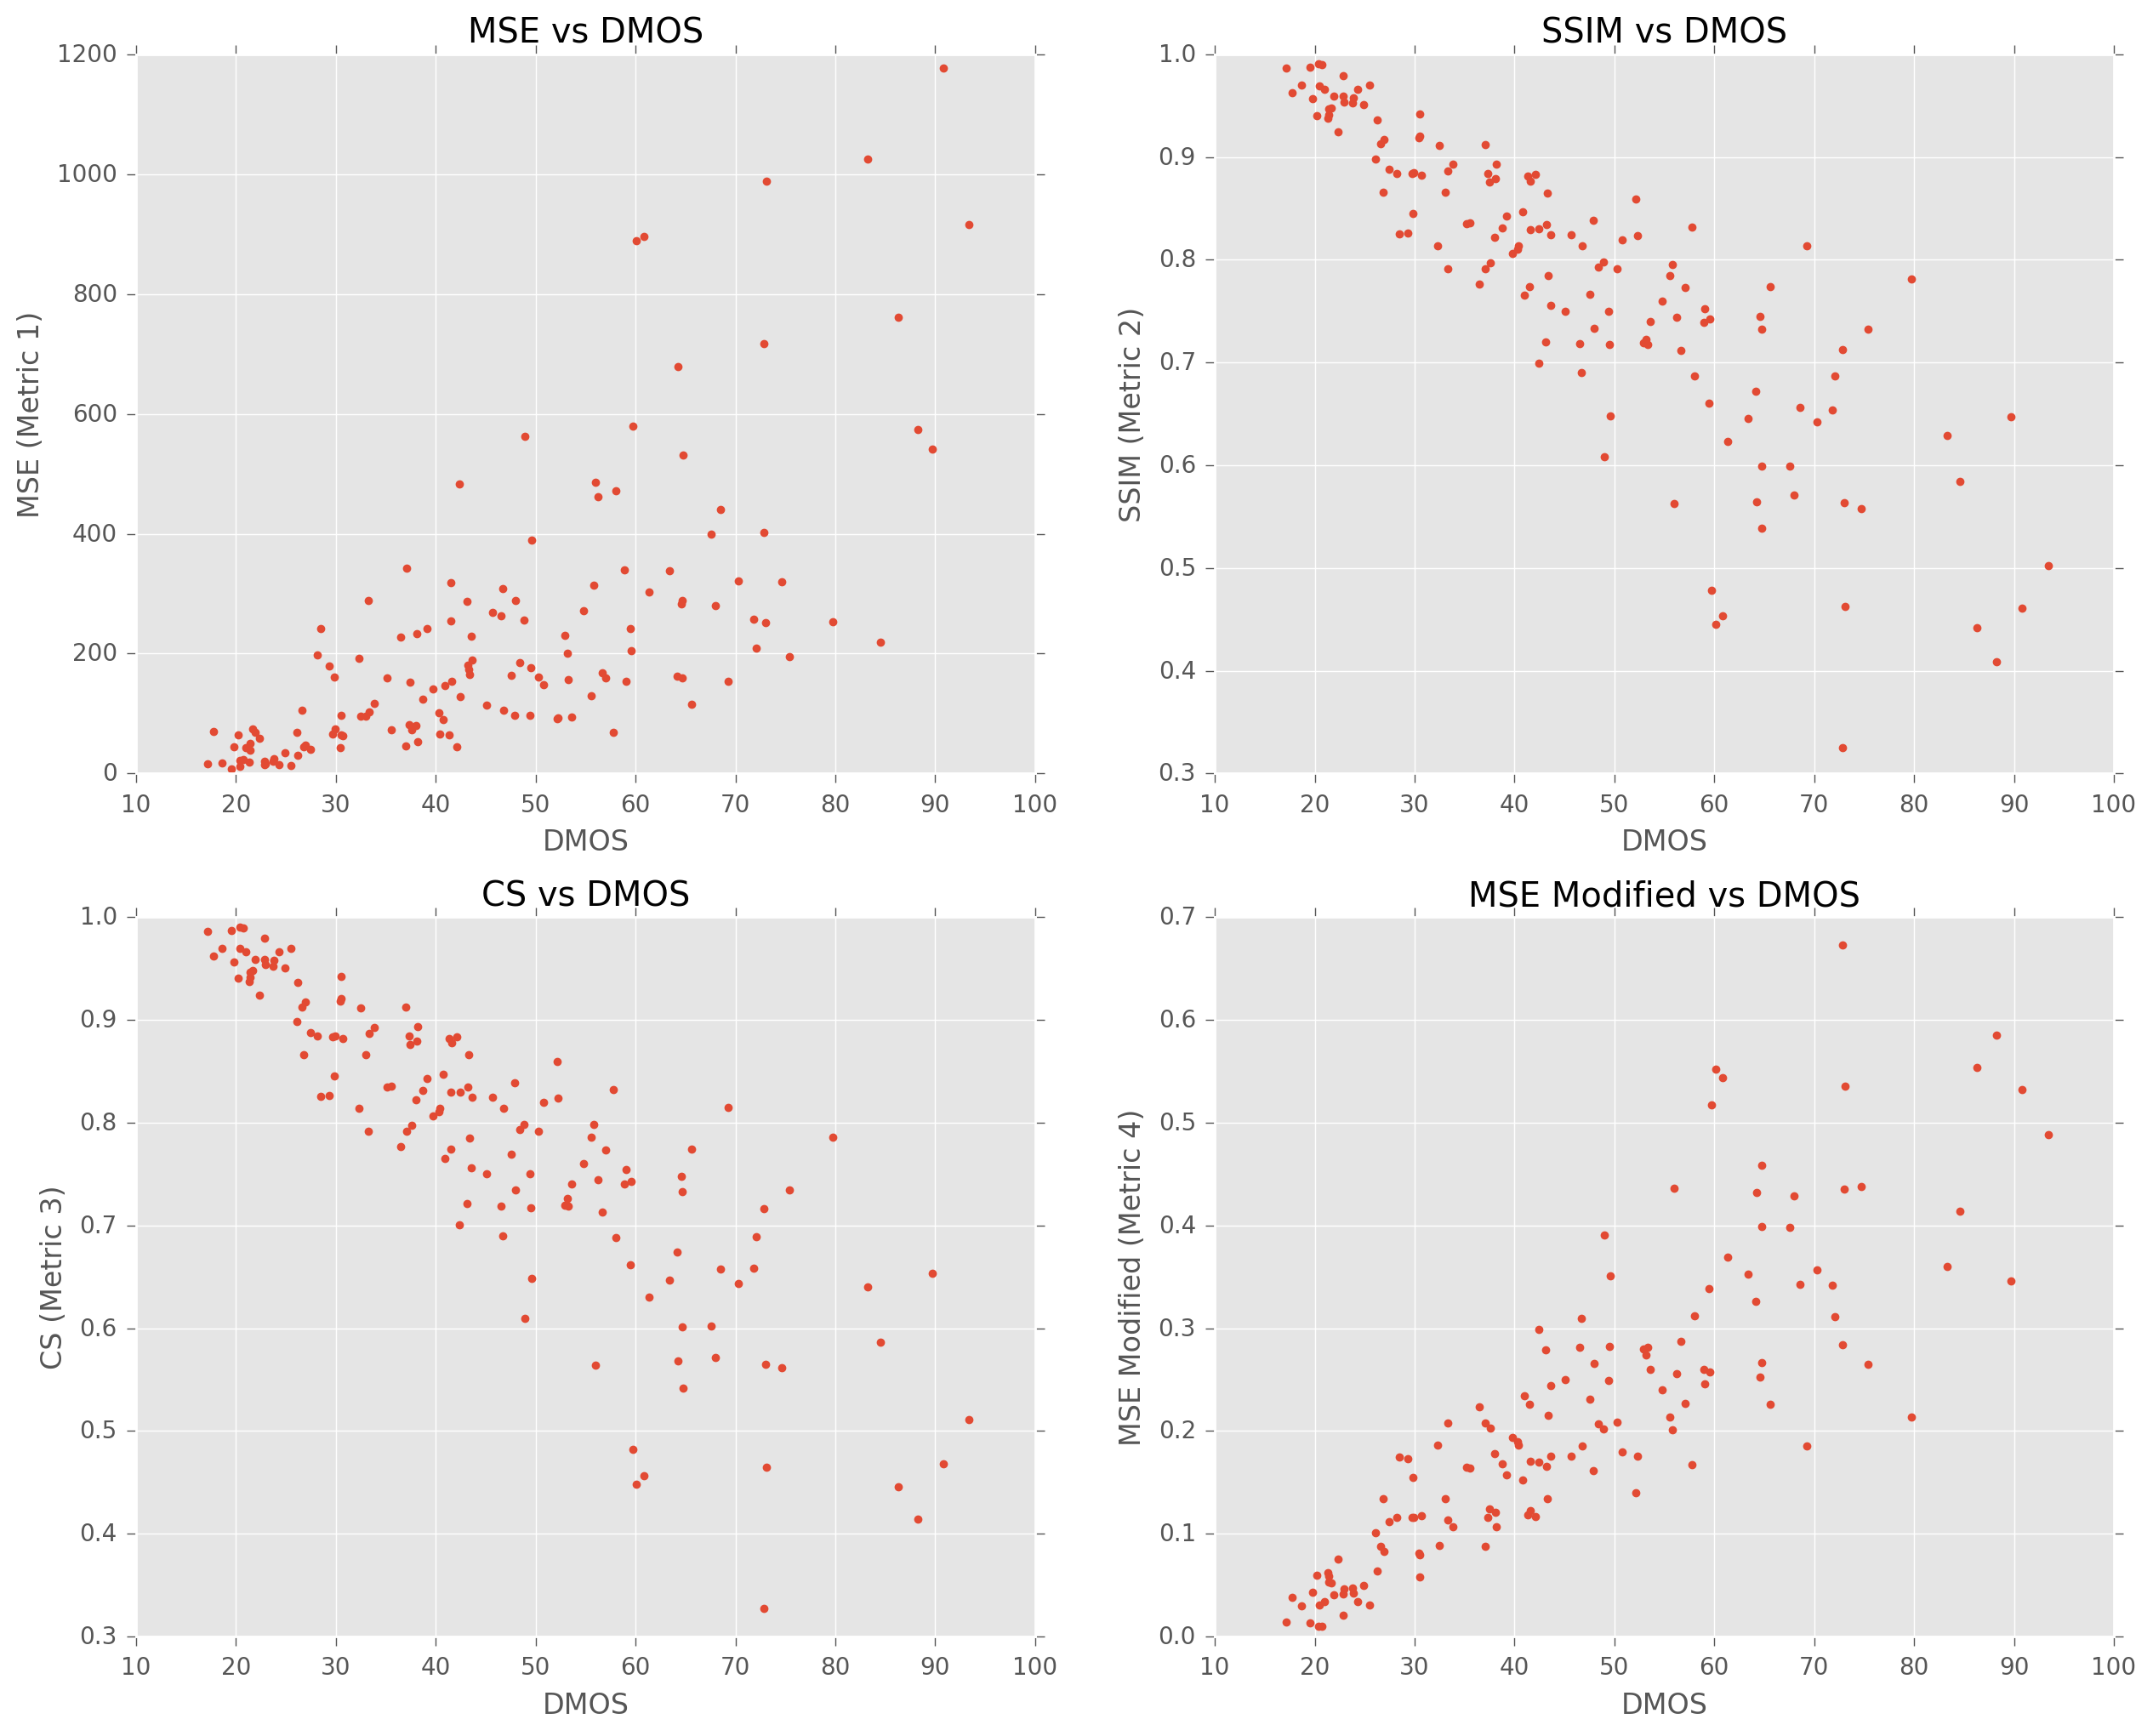
\includegraphics[width=16cm]{../Images/combine_res.png}
			\caption{Comparing DMOS with all metrics}
		\end{figure}
	
		
		\begin{figure}[!htb]
			\centering
			\fbox{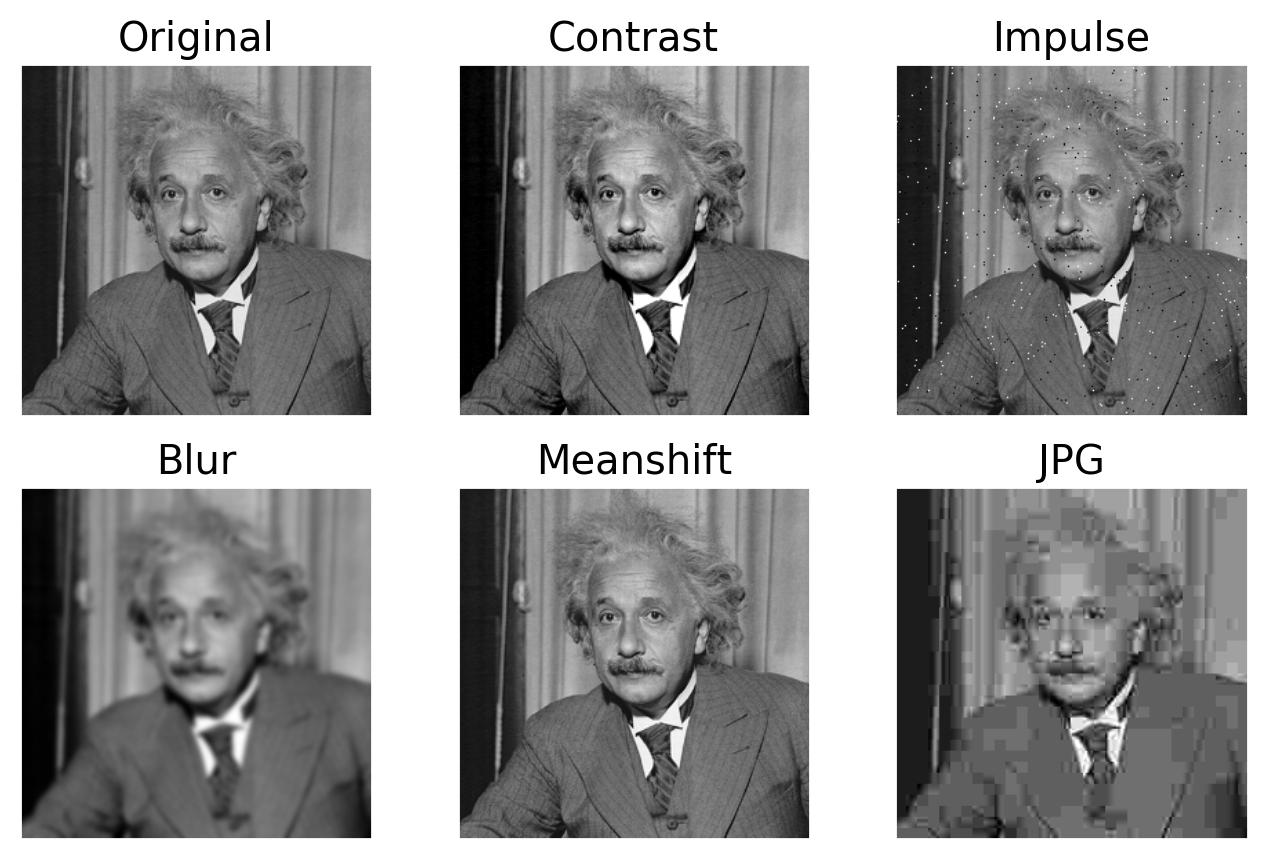
\includegraphics[width=15.5cm]{../Images/compare_img}}
			\caption{Comparing metrics for different distortions}
		\end{figure}

		\begin{table}[b]
			\begin{center}
				\begin{tabular}{||c || c c c c||} 
					\hline 
					& \textbf{MSE} & \textbf{SSIM} & \textbf{CS} & \textbf{MSE$_{mod}$}\\ [0.5ex] 
					\hline \hline
					Contrast & 144.2188 & 0.9012 & 0.9762 & 0.0237 \\ \hline
					Blur & 143.9085 & 0.7022 & 0.7031 & 0.2968 \\ \hline
					Impulse & 143.9390 & 0.8393 & 0.8394 & 0.1605 \\ \hline
					JPG & 141.9529 & 0.6700 & 0.6716 & 0.3283 \\ \hline
					Meanshift & 143.9944 & 0.9873 & 0.9999 & 5.4904e-07 \\ \hline
				\end{tabular}
				\caption{Score of different metrics for images in Figure 2}
			\end{center}
		\end{table}
		
		\newpage
		\subsubsection{Observations:}
		\begin{enumerate}
			\item From the results given in the table we can see that MSE gives the same score for all the images no matter how good or bad the image is. So it is the worst metric among all the gives metrics.
			\item We can see from the result table that smaller the value of MSE$_{mod}$ more closer is the image to the original image. And the opposite holds for the other two metrics SSIM and CS. More closer is their value to 1, more closer is the image to the original.
			\item From the results given in the table, we can see that the sum of the score given by CS and MSE$_{mod}$ is always equal to 1. Therefore, both the metrics are equivalent.
			\item SSIM and CS gives almost the similar results for most of the distortion but their results significantly differ in case of contrast changed image. This is because of the fact that CS is actually SSIM without luminance component.
		\end{enumerate}
	\end{homeworkProblem}
	\newpage
	\begin{homeworkProblem}
		\begin{figure}[!hbt]
			\centering
			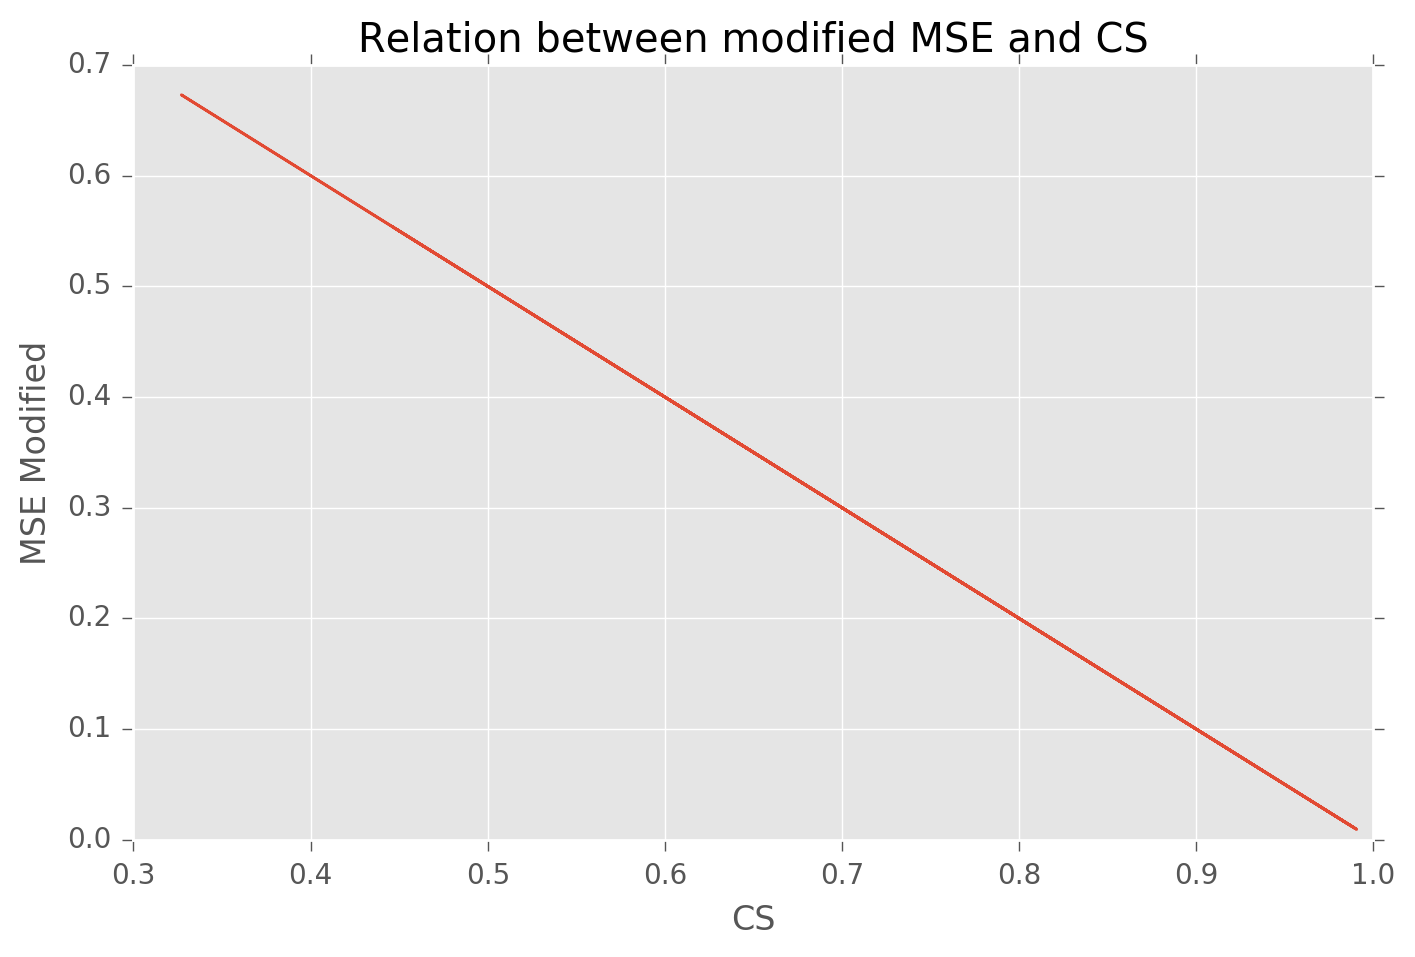
\includegraphics[width=12cm]{../Images/relation.png}
			\caption{Finding relation between CS and MSE$_{mod}$}
		\end{figure}
	
		\subsubsection{Observations:}
		\begin{enumerate}
			\item The graph shows that there exist a linear relation between MSE$_{mod}$ and CS metric. The following derivation proves that the actual relation is:
			$$ MSE_{mod} = 1 - CS$$
		\end{enumerate}
	
	\end{homeworkProblem}
\end{document}